\documentclass[10pt]{../formats/RU}
%%%% delimiters
\DeclarePairedDelimiter\parens{\lparen}{\rparen}
\DeclarePairedDelimiter\bracks{\lbrack}{\rbrack}
\DeclarePairedDelimiter\braces{\lbrace}{\rbrace}
\DeclarePairedDelimiter\abs{\lvert}{\rvert}
\DeclarePairedDelimiter\norm{\lVert}{\rVert}
\DeclarePairedDelimiter\angles{\langle}{\rangle}
\DeclarePairedDelimiter\ceil{\lceil}{\rceil}
\DeclarePairedDelimiter\floor{\lfloor}{\rfloor}

%%%% math operators naming
\DeclareMathOperator*{\argmax}{\textnormal{argmax}}
\DeclareMathOperator*{\argmin}{\textnormal{argmin}}
\DeclareMathOperator{\tr}{\textnormal{tr}}
\DeclareMathOperator{\eig}{\textnormal{eig}}
\DeclareMathOperator{\sgn}{\textnormal{sgn}}
% \let\det\relax % "Undefine" \det
% \DeclareMathOperator{\det}{\textnormal{det}} % already defined in mathtools
\DeclareMathOperator{\diag}{\textnormal{diag}}
\DeclareMathOperator{\rank}{\textnormal{rank}}
\DeclareMathOperator{\Vol}{\textnormal{Vol}}   % volume
\DeclareMathOperator{\Surf}{\textnormal{Surf}} % surface area

%%%% Transforms! -- requires mathtools package
\newcommand*{\LapTrans}{\xleftrightarrow{\mathcal{Z}}}
\newcommand*{\ZTrans}{\xleftrightarrow{\mathcal{L}}}
\newcommand*{\CTFS}{\xleftrightarrow{\textnormal{CTFS}}}
\newcommand*{\CTFT}{\xleftrightarrow{\textnormal{CTFT}}}
\newcommand*{\DTFS}{\xleftrightarrow{\textnormal{DTFS}}}
\newcommand*{\DTFT}{\xleftrightarrow{\textnormal{DTFT}}}

%%%% vector font
\let\oldvec\vec
\renewcommand*{\vec}[1]{\mathbf{#1}}
% \newcommand*{\trn}{\!^{\!\intercal}}
\newcommand*{\trn}{\!^{\mathsf{T}}}
% \newcommand*{\coj}{\!^{\dag}} % Text Mode Symbol, Should not be used
% \newcommand*{\coj}{\!^{\dagger}}
\newcommand*{\coj}{\!^{\mathsf{H}}}
\newcommand*{\inv}{^{-1}}

%%%% number systems
\DeclareMathOperator{\R}{\mathbb{R}}
\DeclareMathOperator{\C}{\mathbb{C}}
\DeclareMathOperator{\N}{\mathbb{N}}
\DeclareMathOperator{\Z}{\mathbb{Z}}
\DeclareMathOperator{\F}{\mathbb{F}}
\DeclareMathOperator{\Q}{\mathbb{Q}}

%%%% STATISTICS AND PROBABILITY
\newcommand*{\Var}{\mathop{\textnormal{Var}}}
\newcommand*{\Cov}{\mathop{\textnormal{Cov}}}
\newcommand*{\Corr}{\mathop{\textnormal{Corr}}}
\newcommand*{\MSE}{\mathop{\textnormal{MSE}}}
\newcommand*{\MSD}{\mathop{\textnormal{MSD}}}
\newcommand*{\NSD}{\mathop{\textnormal{NSD}}}

\newcommand*{\E}[1]{\mathbb{E}\bracks*{#1}}
\newcommand*{\condE}[2]{\mathbb{E}\bracks*{#1 \mid #2}}
\renewcommand*{\P}[1]{\mathbb{P}\parens*{#1}}
\newcommand*{\condP}[2]{\mathbb{P}\parens*{#1 \mid #2}}

\DeclareMathOperator{\Bern}{\mathsf{Bern}}
\DeclareMathOperator{\Unif}{\mathsf{Unif}}
\DeclareMathOperator{\Expv}{\mathsf{Exp}}
\DeclareMathOperator{\Poi}{\mathsf{Poi}}
\DeclareMathOperator{\Gamv}{\mathsf{Gamma}}
\DeclareMathOperator{\Dirv}{\mathsf{Dir}}
\DeclareMathOperator{\Mult}{\mathsf{Mult}}
\DeclareMathOperator{\Beta}{\mathsf{Beta}}
\DeclareMathOperator{\Geomv}{\mathsf{Geom}}
\DeclareMathOperator{\Binomv}{\mathsf{Binom}}
\DeclareMathOperator{\NegBinomv}{\mathsf{NB}}
\DeclareMathOperator{\Lap}{\mathsf{Lap}}
\DeclareMathOperator{\Gaus}{\mathsf{N}}
\DeclareMathOperator{\Weibull}{\mathsf{Weibull}}


\DeclareMathOperator{\iidsim}{\stackrel{\textnormal{i.i.d.}}{\sim}}
\DeclareMathOperator{\diff}{\mathop{}\!\textnormal{d}}

%%%% Special norms and linear algebra stuff
\newcommand*{\subgnorm}[1]{\norm*{#1}_{\psi_2}}
\newcommand*{\subexpnorm}[1]{\norm*{#1}_{\psi_1}}
\newcommand*{\frobnorm}[1]{\norm*{#1}_{\textnormal{F}}}
\newcommand*{\opnorm}[1]{\norm*{#1}_{\textnormal{op}}}
\newcommand*{\Lipnorm}[1]{\norm*{#1}_{\textnormal{Lip}}}

%%%%
\newcommand*{\set}[1]{\braces*{\,#1\,}}
\newcommand*{\ie}{\textnormal{i.e.\ }}
\newcommand*{\eg}{\textnormal{e.g.\ }}
\newcommand*{\etc}{\textnormal{etc.\ }}
\newcommand*{\iid}{\textnormal{i.i.d.\ }}

%Theorem style
\declaretheorem[numbered=no, style=definition]{axiom}
\declaretheorem[numberwithin=section,style=definition]{definition}
\declaretheorem[sibling=definition]{theorem, lemma, corollary, proposition, conjecture}
\declaretheorem[numbered=no,style=remark]{remark, claim}

%Information to be included in the title page:
\title[Random Fourier Feature]{A random matrix analysis of random fourier features}
\subtitle{beyond the Gaussian kernel, a precise phase transition, and the corresponding double descent}
\author[Kai] % (optional, for multiple authors)
{Kailong Wang\inst{1}
%\and Someone Else\inst{2}
}
\institute[Rutgers] % (optional)
{
  \inst{1}%
  Ph.D.\ of ECE\\
  Rutgers University
  % \and
  % \inst{2}%
  % Faculty of Statistics\\
  % Very Famous University
}
\date[\today] % (optional)
{ECE 539 HDP, \today}



\begin{document}
\frame{\titlepage}
%---------------------------------------------------------
%This block of code is for the table of contents after
%the title page
\begin{frame}
\frametitle{Table of Contents}
\tableofcontents
\end{frame}
%---------------------------------------------------------


\section{Motivation}
%---------------------------------------------------------
\begin{frame}
  \frametitle{Linear Classification with Non-linear Input}
  Consider a binary classification problem with non-linear (\eg polynomial) samples. This is not separable with linear function.

  (\eg %$Y=X\beta+b$ where
  $\mathbf{X} = {
    \begin{bmatrix}
      x_{1,1} \ x_{1,2} \\
      x_{2,1} \ x_{2,2} \\
      \cdots \\
      x_{N,1} \ x_{N,2}
    \end{bmatrix}
  }\in \R^{N\times 2}$.)
  \begin{figure}
    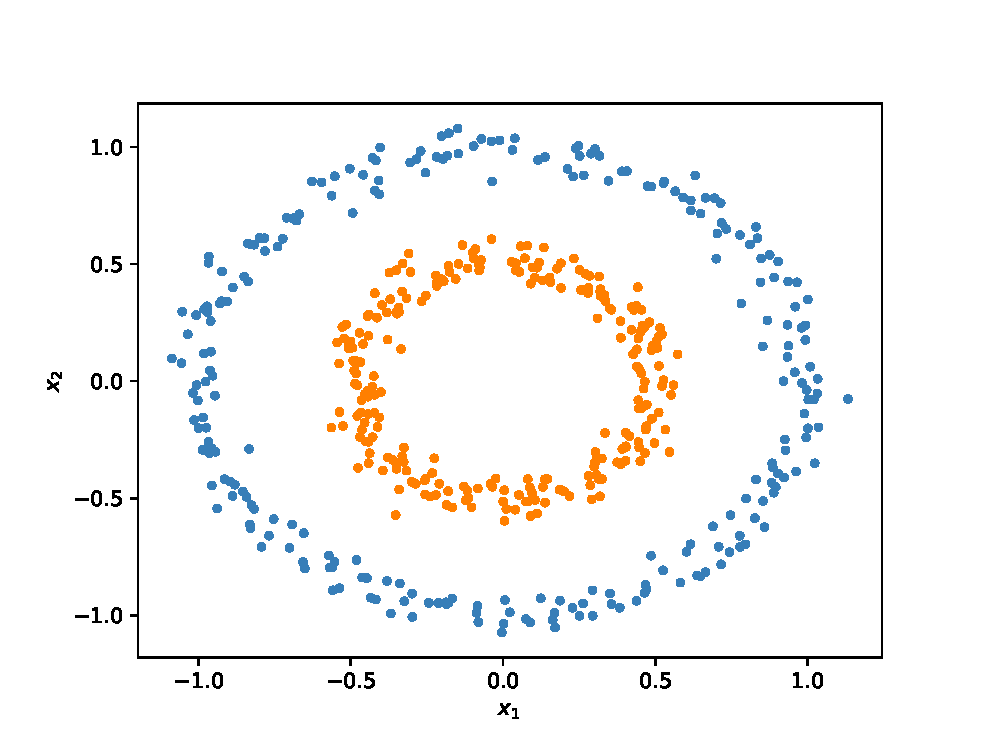
\includegraphics[height=0.5\textheight]{./figs/2d_poly_circle.eps}%
  \end{figure}
\end{frame}
%---------------------------------------------------------
\begin{frame}
  \frametitle{Lifting}
  One idea is to \textbf{LIFT} the samples into a higher dimensional space in which the samples are linearly separable.
  \begin{figure}
    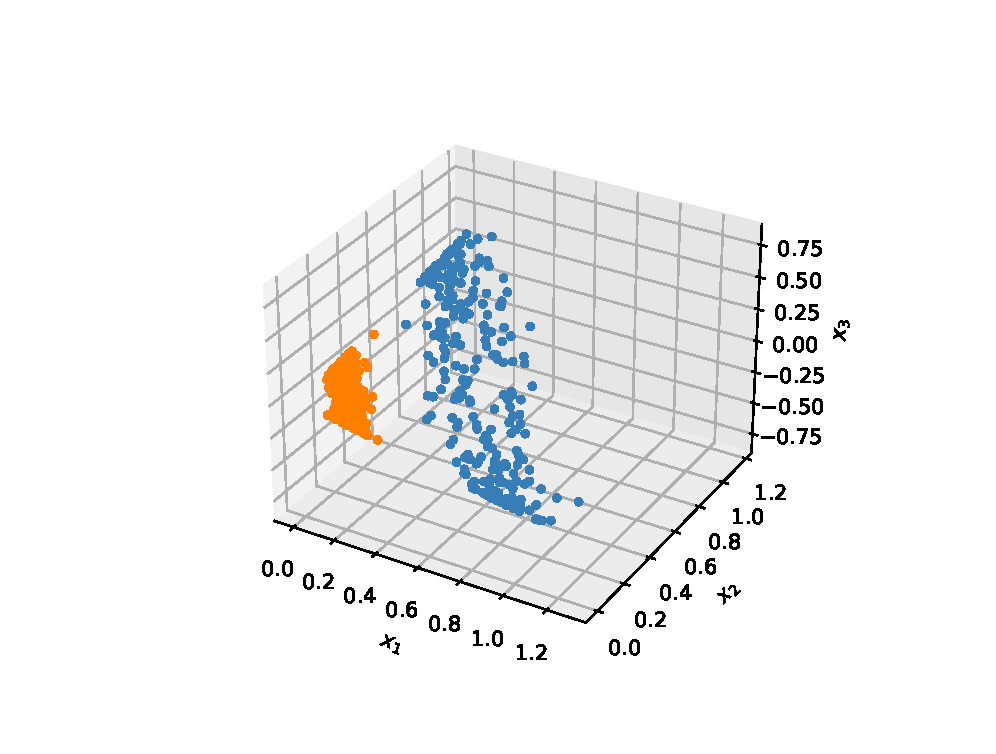
\includegraphics[height=0.45\textheight]{./figs/3d_poly_circle.eps}%
  \end{figure}
  The Lifting function in this case is
  $
  \phi(\mathbf{X}) = {
    \begin{bmatrix}
      x_{1,1}^2 \ x_{1,2}^2 \ \sqrt{2}x_{1,1}x_{1,2} \\
      x_{2,1}^2 \ x_{2,2}^2 \ \sqrt{2}x_{2,1}x_{2,2} \\
      \cdots \\
      x_{N,1}^2 \ x_{N,2}^2 \ \sqrt{2}x_{N,1}x_{N,2}
    \end{bmatrix}
  }
  $.
\end{frame}
%---------------------------------------------------------
\begin{frame}
\frametitle{Curse of Dimensionality}
\begin{itemize}
  \item<1-> Consider solving the above problem with \emph{support vector machine} (SVM).
  \begin{align*}
    \mathcal{L}(\vec{w}, \vec{\alpha}) = \sum_{n=1}^N\alpha_n - \frac{1}{2}\sum_{n}^{N}\sum_{m}^{N}\alpha_n\alpha_m y_ny_m(\mathbf{x_n}\trn \mathbf{x_m}).
  \end{align*}
  The $\vec{w}$ is the linear decision boundary and $\vec{\alpha}$ is a vector of Lagrange multipliers.
  \item <2-> We need to use lifting function $\phi(X)$ to make the samples linearly separable. Specifically, we replace $(\mathbf{x_n}\trn \mathbf{x_m})$ with $(\phi(\mathbf{x_n})\trn\phi(\mathbf{x_m}))$.
  \begin{align*}
    \phi(\mathbf{x_n})\trn\phi(\mathbf{x_m})
    &= \bracks*{x_{n,1}^2 \ x_{n,2}^2 \ \sqrt{2}x_{n,1}x_{n,2}}\bracks*{x_{m,1}^2 \ x_{m,2}^2 \ \sqrt{2}x_{m,1}x_{m,2}}\trn \\
    &= x_{n,1}^2x_{m,1}^2 + x_{n,2}^2x_{m,2}^2 + 2x_{n,1}x_{n,2}x_{m,1}x_{m,2}
  \end{align*}
  \item<3-> Calculate the inner product in the $\R^3$ across all $N$ pairs of samples is acceptable. However, the lifting function $\phi(X)$ is usually very high dimensional.
\end{itemize}
\end{frame}
%---------------------------------------------------------
\begin{frame}
  \frametitle{Kernel Trick}
  \begin{itemize}
    \item <1-> Consider the following derivation,
    \begin{align*}
      (\mathbf{x_n}\trn \mathbf{x_m})^2
      &= \parens*{\bracks*{x_{n,1} \ x_{n,2}}\bracks*{x_{m,1} \ x_{m,2}}\trn}^2 \\
      &= \parens*{x_{n,1}x_{m,1} + x_{n,2}x_{m,2}}^2 \\
      &= x_{n,1}^2x_{m,1}^2 + x_{n,2}^2x_{m,2}^2 + 2x_{n,1}x_{n,2}x_{m,1}x_{m,2} \\
      &= \phi(\mathbf{x_n})\trn\phi(\mathbf{x_m})
    \end{align*}
    \item <2-> Instead of computing inner product in the high dimensional space, we compute the inner product in the original space.
    \item <3-> The function
    \begin{align*}
      K(\mathbf{x_n}, \mathbf{x_m}) = (\mathbf{x_n}\trn \mathbf{x_m})^2 = \phi(\mathbf{x_n})\trn\phi(\mathbf{x_m})
    \end{align*}
     is called a \textbf{kernel function}.
  \end{itemize}
\end{frame}
%---------------------------------------------------------
\begin{frame}
  \frametitle{There must be disadvantages\ldots}
  \begin{itemize}
    \item <1-> Given training data $(\vec{x_1}, y_1), (\vec{x_2}, y_2), \ldots, (\vec{x_N}, y_N) \in \mathcal{X}\times\mathcal{Y}$, where $\mathcal{X}\subseteq \R^d$ and $\mathcal{Y}\subseteq\R$. Consider \emph{Kernel Ridge Regression} (KRR), with $\phi(\mathcal{X})\subseteq \R^k$, where $k\rightarrow\infty$
    \begin{align*}
      \mathcal{L}(\vec{w}, \lambda)=\argmin_{\vec{w}}\sum_{n}^{N}(y_n - \vec{w}\trn\phi(\vec{x}_n))^2 + \lambda\vec{w}\trn\vec{w}.
    \end{align*}
    Solving it with Lagrange multipliers $\vec{\alpha}$, which is the solution of
    \begin{align*}%\label{}
      (\mathbf{K}+\lambda\mathbf{I}_k)\vec{\alpha} = \vec{y},
    \end{align*}
    requires $\Theta(k^3)$ time and $\Theta(k^2)$ memory. Here $\mathbf{K}\in \R^{k\times k}$ is the kernel matrix or Gram matrix defined by $\mathbf{K}_{nm} \equiv K(\mathbf{x_n}, \mathbf{x_m})$.
    \item <2-> \textbf{Intuition:} Can we find a kernel function which lifts $\mathcal{X}$ to $\R^s$, where $d < s\ll k$, while not sacrifices model performance?
  \end{itemize}
\end{frame}
%---------------------------------------------------------


\section{Random Fourier Features}
%---------------------------------------------------------
\begin{frame}
\frametitle{Some Prerequisites}
\begin{alertblock}{Shift Invariant Kernel (Radial Basis Function (RBF))}
  A kernel function $K(\vec{x_n}, \vec{x_m})$ is called \textbf{shift invariant} if it can be written as $K(\vec{x_n}, \vec{x_m}) = g(\vec{x_n}-\vec{x_m})$ for some function $g(\cdot)$

  (\eg $K_{Gaussian}(\vec{x_n},\vec{x_m})=\exp(-\gamma\norm{\vec{x_n}-\vec{x_m}}_2^2)$).
\end{alertblock}
\begin{block}{Mercer’s Theorem}
  A continuous function $K(\vec{x_n}, \vec{x_m})$ is a valid kernel function if and only if the kernel matrix $\mathbf{K}$ is \textbf{positive semi-definite}.
\end{block}
\begin{block}{Bochner's Theorem}
  A continuous function $g(\cdot)$ is \textbf{positive semi-definite} if and only if it is the Fourier transform of a non-negative measure.
\end{block}
\end{frame}
%---------------------------------------------------------
\begin{frame}
  \frametitle{Random Fourier Features}
  \begin{exampleblock}{Conclusion}
    A continuous \textbf{shift invariant} kernel $K(\vec{x_n}, \vec{x_m})$, which is \textbf{positive semi-definite} (Mercer's Theorem), is the Fourier transform of a non-negative measure $p(\cdot)$.
    \begin{align}
      \phi(\vec{x_n})\trn\phi(\vec{x_m})
      &= K(\vec{x_n}, \vec{x_m}) = K(\vec{x_n}-\vec{x_m}) \\
      &=\int_{\R^d}p(\vec{\omega})\exp(i\vec{\omega}\trn(\vec{x_n}-\vec{x_m}))d\vec{\omega} \\
      &= \mathbb{E}_{\vec{\omega}}\bracks*{\xi_{\vec{\omega}}(\vec{x_n})^*\xi_{\vec{\omega}}(\vec{x_m})}\label{rffinC}
    \end{align}
    Here
    $
    \xi_{\vec{\omega}}(\vec{x})=\exp(i\vec{\omega}\trn\vec{x})
    ={
      \begin{bmatrix}
        \cos(\vec{\omega}\trn\vec{x}) \\
        \sin(\vec{\omega}\trn\vec{x})
      \end{bmatrix}
    }
    $
    and hence $\xi_{\vec{\omega}}(\vec{x_n})^*\xi_{\vec{\omega}}(\vec{x_m})$ is an unbiased estimator of $K(\vec{x_n}, \vec{x_m})$ when $\vec{\omega}$ is drawn from $p(\cdot)$.
  \end{exampleblock}
\end{frame}
%---------------------------------------------------------
\begin{frame}
  \frametitle{Random Fourier Features}
  \begin{itemize}
    \item <1-> Since both the $p(\cdot)$ and $K(\triangle)$ are real-valued, we can replace $\xi_{\vec{\omega}}(\vec{x})$ with $z_{\vec{\omega}}(\vec{x})=[\sqrt{2}\cos(\vec{\omega}\trn\vec{x}+b)]$ where $\vec{\omega}$ is drawn from $p(\vec{\omega})$ and $b$ is uniformly drawn from $[0, 2\pi]$. Then eq.~\eqref{rffinC} becomes $\mathbb{E}_{\vec{\omega}}[z_{\vec{\omega}}(\vec{x_n})\trn z_{\vec{\omega}}(\vec{x_m})]$
    \item <2-> \textbf{Note:} $z_{\vec{\omega}}(\vec{x_n})\trn z_{\vec{\omega}}(\vec{x_m})$ is an unbiased estimator of $\phi(\vec{x_n})\trn\phi(\vec{x_m})$. The $z_{\vec{\omega}}(\vec{x})$ is not a lifting function.
    \item <3-> \textbf{Note:} To further reduce the variance of the estimator, we can randomly draw $s$ samples of $\vec{\omega}$ and normalize each corresponding $z_{\vec{\omega}}(\vec{x})$ by $\sqrt{s}$. Then the inner product $z(\vec{x_n})\trn z(\vec{x_m})=\frac{1}{s}\sum_{j=1}^{s}z_{\vec{\omega}j}(\vec{x_n})\trn z_{\vec{\omega}j}(\vec{x_m})$
    % \item <4-> \textbf{Question:} The author samples $\vec{\omega}$ from $\R^d$ and average over $s$ samples in the following algorithm. However, $d\&s$ seems can be arbitrary number based on the above derivation.
  \end{itemize}
\end{frame}
%---------------------------------------------------------
\begin{frame}
  \frametitle{Algorithm}
  \begin{algorithm}[H]
    \caption{Random Fourier Features}\label{RFF}
    \begin{algorithmic}
    \Require A shift invariant kernel $K(\vec{x_n}, \vec{x_m}) = K(\vec{x_n}- \vec{x_m})$.
    \Ensure A randomized feature map $z(\vec{x}): \R^d\rightarrow\R^s$ so that $z(\vec{x_n})\trn z(\vec{x_m})\approx K(\vec{x_n}, \vec{x_m})$.
    \State Compute the Fourier transform $p(\cdot)$ of the kernel $K: p(\vec{\omega})=\frac{1}{2\pi}\int \exp(-i\vec{\omega}\trn\triangle)K(\triangle)\diff\triangle$
    \State Draw $s$ \iid samples $\vec{\omega}_1, \vec{\omega}_2, \ldots, \vec{\omega}_s \in \R^d$ from $p(\cdot)$ and $s$ \iid samples $b_1, b_2, \ldots, b_s \in [0, 2\pi]$.
    \State Let $z(\vec{x})\equiv \sqrt{\frac{2}{s}}[\cos(\vec{\omega}_1\trn\vec{x}+b_1)\ \cos(\vec{\omega}_2\trn\vec{x}+b_2)\ \ldots\ \cos(\vec{\omega}_s\trn\vec{x}+b_s)]\trn$
    \end{algorithmic}
  \end{algorithm}
\end{frame}
%---------------------------------------------------------
\begin{frame}
  \frametitle{Convergence}
  \begin{exampleblock}{Bound for a \emph{fixed} pair of samples $\vec{x_n}$ and $\vec{x_m}$}
    Given $z_{\vec{\omega}}$ is bounded random variable between $[-\sqrt{2}, \sqrt{2}]$, with Hoeffding's Inequality, we have
    \begin{align*}
      \P{\abs{z(\vec{x_n})\trn z(\vec{x_m})-K(\vec{x_n}, \vec{x_m})}\geq \epsilon} \leq 2\exp\parens*{-\frac{s\epsilon^2}{4}}.
    \end{align*}
  \end{exampleblock}
\end{frame}
%---------------------------------------------------------
\begin{frame}
  \frametitle{Convergence}
  \begin{exampleblock}{Bound for \emph{all} pair of samples $\vec{x_n}$ and $\vec{x_m}$}
    Let $\mathcal{M}$ be a compact sunset of $\R^d$ with diameter $\textnormal{diam}(\mathcal{M})$. Then, for the mapping $z$ defined in Algorithm~\ref{RFF}, we have
    \begin{align*}
      \P{\sup_{x,y\in\mathcal{M}}\abs{z(\vec{x_n})\trn z(\vec{x_m})-K(\vec{x_n}, \vec{x_m})}\geq \epsilon} \\
      \leq 2^8\parens*{\frac{\sigma_{p(\cdot)}\textnormal{diam}(\mathcal{M})}{\epsilon}}^2\exp\parens*{-\frac{s\epsilon^2}{4(d+2)}}.
    \end{align*}
  \end{exampleblock}
\end{frame}
%---------------------------------------------------------
\begin{frame}{Common RFF}
  \centering
  \begin{tabular}{c c c}
    Kernel & $K(\triangle)$ & $p(\vec{\omega})$ \\
    \hline
    Gaussian & $\exp(-\gamma\norm{\triangle}_2^2)$ & $(2\pi)^{-\frac{s}{2}}\exp{-\gamma\norm{\vec{\omega}}_2^2}$\\
    Laplacian & $\exp(-\norm{\triangle}_1)$ & $\prod\limits_{d}(\pi(1+\omega_d^2))^{-1}$\\
    Cauchy & $\prod\limits_{d}2(1+\triangle_d^2)^{-1}$ & $\exp(-\norm{\triangle}_1)(\textcolor{red}{\mathord{?}})$
  \end{tabular}
\end{frame}
%---------------------------------------------------------

\section{An analysis of RFF}
%---------------------------------------------------------
\begin{frame}
  \frametitle{The challenge that RFF faces in the learning regime}
  Consider a machine learning system with $d$ parameters, trained on a dataset of size $N$, asymptotic analysis has
  \begin{itemize}
    \item \textbf{Classical regime:} either focuses on the (statistical) population $N\rightarrow\infty$ limit, for $d$ fixed, or the over-parameterized $d\rightarrow\infty$ limit, for a given $N$.
    \item \textbf{Modern regime:} modern learning system (\eg Neural Network) usually has model complexity and data size increase together. A double asymptotic regime where $N, d\rightarrow\infty, d/N\rightarrow c$ is established.
  \end{itemize}
  RFF has been shown that entry-wise the Gram matrix $\xi(\vec{x})$ converges to the Gaussian kernel matrix as $s\rightarrow\infty$ and this property remains in modern regime.

  However, the convergence $\norm{\mathbf{\Xi}\trn\mathbf{\Xi}/s-\mathbf{K}}\rightarrow 0$ no longer holds in spectral norm (blow-up). Here $\mathbf{\Xi}$ is the matrix formed by stacking $\xi(\vec{x})$ for all samples.
\end{frame}
%---------------------------------------------------------
\begin{frame}
  \frametitle{Setup}
  \begin{itemize}
    \item $0< \lim\inf\limits_N\min\braces{\frac{s}{N},\frac{d}{N}}\leq \lim\sup\limits_N\max\braces{\frac{s}{N},\frac{d}{N}}<\infty$.
    \item $\lim\sup\limits_N\norm{\mathbf{X}}_2<\infty \qquad \lim\sup\limits_N\norm{\vec{y}}_{\infty}<\infty$
    \item In classical regime $\norm{\mathbf{\Xi}\trn\mathbf{\Xi}/s}\equiv \mathbf{K}\equiv\mathbf{K}_{\cos}+\mathbf{K}_{\sin}$
    \item Training MSE: $\mathcal{L}_{train}=\frac{1}{N}\norm{\vec{y}-\mathbf{\Xi}\trn\vec{w}}_2^2=\frac{\lambda^2}{N}\norm{\mathbf{Q}(\lambda)\vec{y}}_2^2$ where
    \begin{align*}
      \mathbf{Q}(\lambda)\equiv\parens*{\frac{1}{N}\mathbf{\Xi}\trn\mathbf{\Xi}+\lambda\mathbf{I}_N}^{-1}
    \end{align*}
    \item We want to assess the asymptotic $\mathcal{L}_{train}$ by expectation which is equivalent to assess the asymptotic $\mathbb{E}_{\vec{\Omega}}\braces{\mathbf{Q}(\lambda)}$ where $\vec{\Omega}$ is the matrix form of $\vec{\omega}$, which is numerically hard.
    % \item Testing MSE: $\mathcal{L}_{test}=\frac{1}{N}\norm{\vec{\hat{y}}-\mathbf{\hat{\Xi}}_{test}\trn\vec{w}}_2^2$
    \item \textbf{Object:} Find an asymptotic ``alternative'' for $\mathbb{E}_{\vec{\Omega}}\braces{\mathbf{Q}(\lambda)}$ when $d, s, N\rightarrow\infty$.
  \end{itemize}
\end{frame}
%---------------------------------------------------------
\begin{frame}
  \frametitle{Some Vague Idea from me...}
  We want to show that with consideration of $d, s, N$
  \begin{align*}
    &\norm{\mathbb{E}_{\vec{\Omega}}\braces{\mathbf{Q}(\lambda)}-\mathbf{\hat{Q}}(\lambda)}_2\rightarrow 0 \\
    &\mathbf{\hat{Q}}(\lambda)\equiv\parens*{\frac{s}{N}\parens*{\frac{\vec{K}_{\cos}}{1+\delta_{\cos}}+\frac{\vec{K}_{\sin}}{1+\delta_{\sin}}}+\lambda\mathbf{I}_N}^{-1} \\
    &\delta_{\cos}=\frac{1}{N}\tr\parens*{\vec{K}_{\cos}\vec{\hat{\vec{Q}}}} \qquad \delta_{\sin}=\frac{1}{N}\tr\parens*{\vec{K}_{\sin}\vec{\hat{\vec{Q}}}}
  \end{align*}
  When $\frac{s}{N}\rightarrow\infty$, $\delta_{\cos},\delta_{\sin}\rightarrow 0$ and thus $\mathbf{\hat{Q}}\simeq \parens*{\frac{s}{N}\mathbf{K}}^{-1}$
\end{frame}
%---------------------------------------------------------

\end{document}